\section{More empirical analyses}

\subsection{Epoch-wise double descent is ubiquitous in adversarial training}
% \subsection{Reconcile robust overfitting and epoch-wise double descent}
\label{sect:double-descent-reconcile}

% In this section, we conduct extensive experiments with different optimizers, sample sizes, model architectures, and learning rate schedulers to verify the connection between robust overfitting and epoch-wise double descent. The default experiment settings are listed in Appendix~\ref{sect: exp-double-descent} in detail.

In this section, we conduct extensive experiments with different model architectures, and learning rate schedulers to verify the connection between robust overfitting and epoch-wise double descent. The default experiment settings are listed in Appendix~\ref{sect: exp-double-descent} in detail.


% We focus on PGD training as it is simple in nature and can produce robustness comparable to state-of-the-art methods~\cite{Rice2020OverfittingIA, pang2021bag, Gowal2020UncoveringTL}.

% \smallsection{Optimizer}
% Similar to the setting employed in \citet{Nakkiran2020DeepDD}, we conduct the adversarial training using both the Adam optimizer and SGD. As already shown in Figure~\ref{fig:intro}, double descent can be observed for both optimizers, although Adam may be inferior compared to SGD.


% \smallsection{Sample size}
% We randomly sample a desired number of examples without replacement from the original training set in CIFAR-10. As shown in Figure \ref{fig:reconcile-sample-size}, for both optimizers, increasing sample size will shrink the area under the double descent curve, but will not significantly distort its shape. 
% % reduce the overfitting gap, defined by the difference between the intermediate minimum and intermediate maximum of the robust test error.
% Similar observation is also made for double descent curve under standard training~\citep{Nakkiran2020DeepDD}.

% \begin{figure*}[!ht]
%   \centering
%   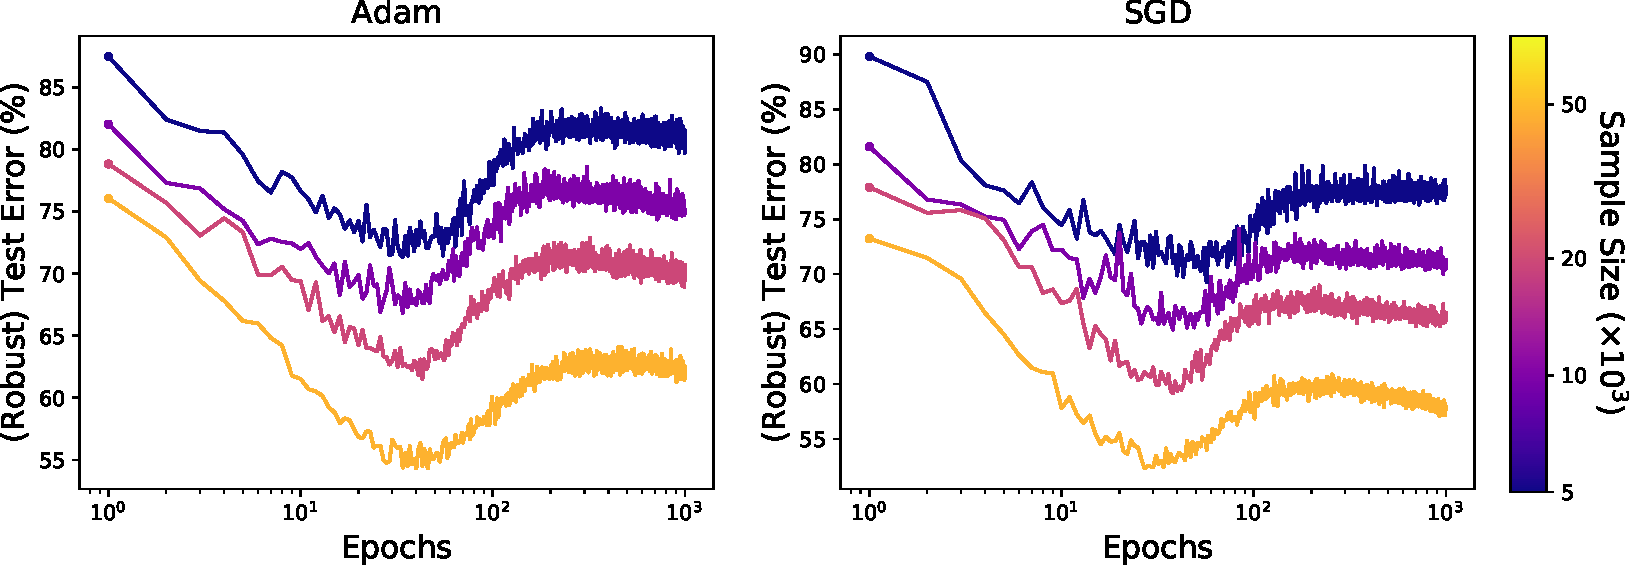
\includegraphics[width=0.9\textwidth]{figures/reconcile-sample-size.pdf}
%   \caption{Varying sample size will shrink the area under the epoch-wise double descent curve, but will not significantly distort its shape.
%   }
% \label{fig:reconcile-sample-size}
% \end{figure*}

% \subsection{Model, learning rate scheduler and regularization}

% \chengyu{Figure: Four subfigures side by side}


\smallsection{Model capacity}
We modulate the capacity of the deep model by varying the widening factor of the Wide ResNet. To extend the lower limit of the capacity, we allow the widening factor to be less than $1$. In such case, the number of channels in each residual block is scaled similarly but rounded, and the number of channels in the first convolutional layer will be reduced accordingly to ensure the width monotonically increasing through the forward propagation. 
% To accelerate the training with an extremely large model, we randomly sample a training set of size $5000$ and employ the Adam optimizer, since the sample size will not significantly distort the shape of the double descent as shown above. Figure~\ref{fig:reconcile-model-capacity} shows that the double descent will gradually become more complete as the model capacity increases and the model translates from under-parameterized to over-parameterized regime~\citep{Nakkiran2020DeepDD}.


\begin{figure*}[!ht]
\centering
\begin{subfigure}[t]{.48\textwidth}
  \centering
  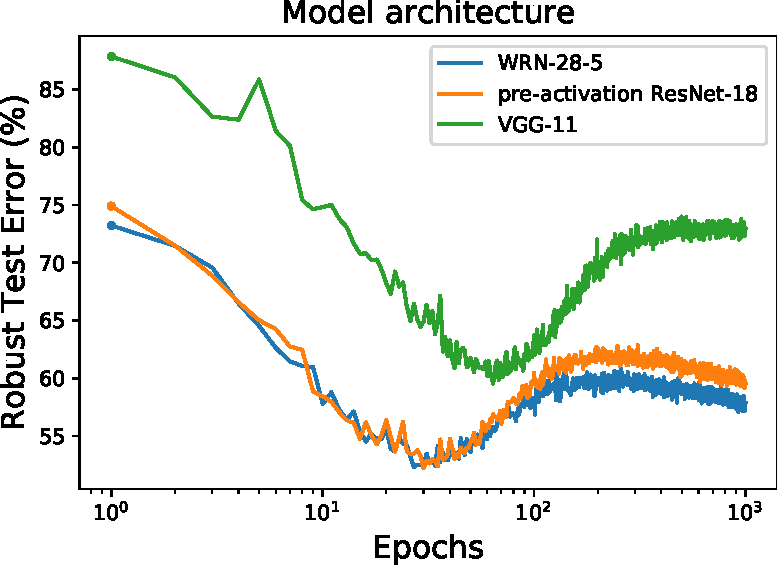
\includegraphics[width=.95\textwidth]{figures/reconcile-model-architecture.pdf}
  \caption{
  % Different model architectures will affect the double descent curve. In particular, VGG-11 will have the second descent delayed due to its inferior performance compared to residual architectures.
  Epoch-wise double descent curves in adversarial training with various model architectures.
  }
  \label{fig:reconcile-model-architecture}
\end{subfigure}\hfill
\begin{subfigure}[t]{.48\textwidth}
  \centering
  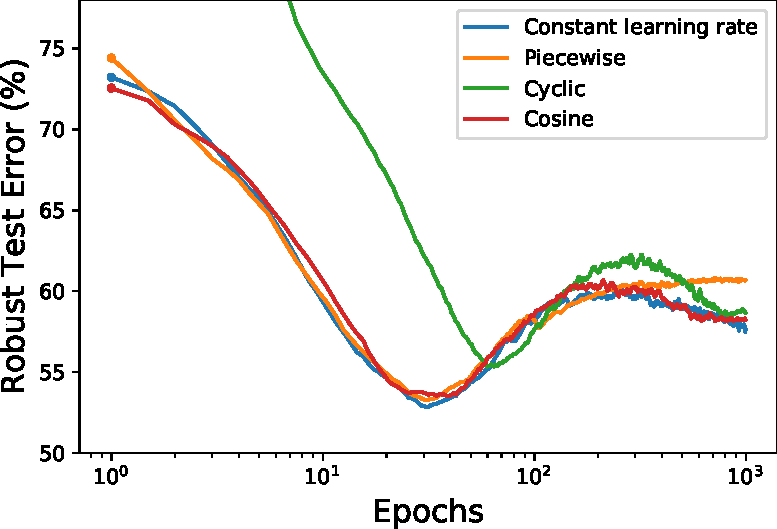
\includegraphics[width=0.95\textwidth]{figures/reconcile-lr-scheduler.pdf}
  \caption{
  % The effect of the learning rate scheduler on the epoch-wise double descent curve in adversarial training. Modulating the model capacity can produce training curves with diverse behaviors. Different model architectures may produce slightly different double descent curves. 
   Epoch-wise double descent curves in adversarial training with various learning rate schedulers.
   The curves are smoothed by a moving average with a window of $5$ to avoid overlapping.
  }
\label{fig:reconcile-lr-scheduler}
\end{subfigure}
  \caption{Effect of model on the epoch-wise double descent curve}
 \label{fig:reconcile-model}
\end{figure*}

% \begin{figure*}[!ht]
%   \centering
%   \includegraphics[width=0.9\textwidth]{figures/reconcile-model.pdf}
%   \caption{The effect of the model architecture on the epoch-wise double descent curve in adversarial training. Modulating the model capacity can produce training curves with diverse behaviours. Different model architectures may produce slightly different double descent curves. The training curve is smoothed by moving average with a window of $5$.
%   }
% \label{fig:reconcile-model}
% \end{figure*}

% As proposed for double descent under standard training, both increasing the model capacity and training longer will increase the effective model complexity (EMC)~\citep{Nakkiran2020DeepDD}, thus driving the model from under-parameterized regime to over-parameterized regime. Indeed, as shown in Figure \ref{fig:reconcile-model}, modulating the capacity of the model can produce diverse behaviours of the training curve. For fairly small models, even the ascent interval will not be observed thus the robust test error will monotonically decrease throughout the training. For moderately large models, the ascent interval is observed thus the robust test error will increase after a certain point during training, which is the typical case present in adversarial training practice and known as robust overfitting. Finally, for sufficiently large model, a more complete picture of the double descent can be observed. Therefore the robust test error will decrease again after the robust overfitting. We note that due to computational constraints, we cannot capture the entire second descent interval, wherefore whether the minimum achieved in the second descent will be better than the first minimum is not clear. Nevertheless, under certain circumstances, such as with smaller perturbation radius or better data quality, we can indeed observe a better second minimum, which will be discussed in Section \ref{sect:factor}.

% In addition, increasing the capacity will also gradually shrink the overfitting gap. One may imagine that sufficiently large model will not undergo double descent and the robust overfitting will not happen likewise. We indeed observe this under certain circumstances as shown in Section \ref{sect:factor}.

\smallsection{Model architecture} We also experiment on model architectures other than Wide ResNet, including pre-activation ResNet-18~\citep{He2016IdentityMI} and VGG-11~\citep{Simonyan2015VeryDC}. We select these configurations to ensure comparable model capacities\footnote{WRN-28-5, pre-activation ResNet-18 and VGG-11 have $9.13\times 10^6$, $11.17\times 10^6$ and $9.23\times 10^6$ parameters, respectively.}. As shown in Figure \ref{fig:reconcile-model}, different model architectures may produce slightly different double descent curves. The second descent of VGG-11 in particular will be delayed due to its inferior performance compared to residual architectures.

% \smallsection{Optimizer}

% \smallsection{Method}
% \chengyu{Maybe method is more important that regularization}

\smallsection{Learning rate scheduler}
% \chengyu{maybe put the figure to appendix}
A specific learning rate scheduler may shape the robust overfitting differently as suggested by \citet{Rice2020OverfittingIA}. We consider the following learning rate schedulers in our experiments.
\begin{itemize}[leftmargin=*]
    \item \textbf{Piecewise decay}: The initial learning rate rate is set as $0.1$ and is decayed by a factor of $10$ at the $100$th and $500$th epochs within a total of $1000$ epochs.
    \item \textbf{Cyclic}: This scheduler was initially proposed by \citet{Smith2017CyclicalLR} and has been popular in adversarial training. We set the maximum learning rate to be $0.2$, and the learning rate will linearly increase from $0$ to $0.2$ for the initial $400$ epochs and decrease to $0$ for the later $600$ epochs.
    \item \textbf{Cosine}: This scheduler was initially proposed by \citet{Loshchilov2017SGDRSG}. The learning rate starts at $0.1$ and gradually decrease to $0$ following a cosine function for a total of $1000$ epochs.
\end{itemize}
Experiments on various learning rate schedulers show the second descent can be widely observed except the piecewise decay, where the appearance of second descent might be delayed due to extremely small learning rate in the late stage of training. 
% This further demonstrates the connection between robust overfitting and epoch-wise double descent.

% \label{sect: exp-lr-scheduler}
% \todo{merge with above}
% For SGD specifically, we also consider the following types of learning rate scheduler to align with \citet{Rice2020OverfittingIA}.


% \begin{figure*}[!ht]
%   \centering
%   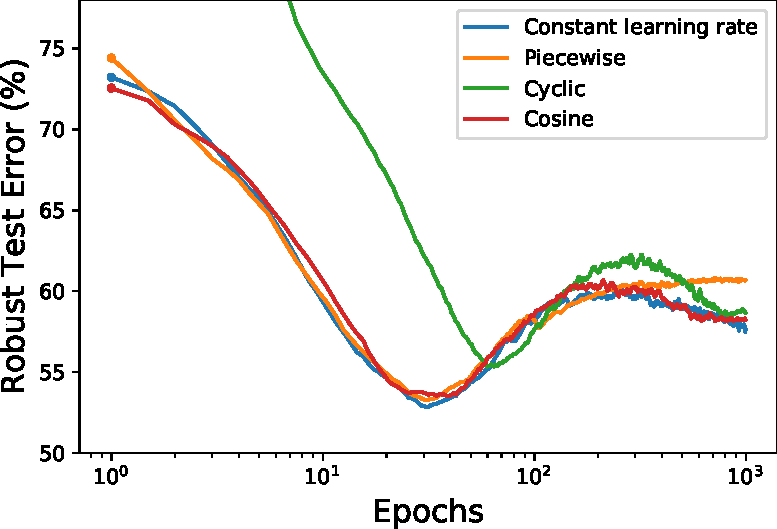
\includegraphics[width=0.45\textwidth]{figures/reconcile-lr-scheduler.pdf}
%   \caption{The effect of the learning rate scheduler on the epoch-wise double descent curve in adversarial training. Modulating the model capacity can produce training curves with diverse behaviors. Different model architectures may produce slightly different double descent curves. The training curve is smoothed by moving average with a window of $5$.
%   }
% \label{fig:reconcile-lr-scheduler}
% \end{figure*}

% \smallsection{Regularization}
% \subsection{\chengyu{Bias-variance analysis of adversarial training}}


% version https://git-lfs.github.com/spec/v1
oid sha256:21e6d7ec228b1a541a47be7af0bd934ed9a0f34a1749875e562206e0445a39f9
size 9061

% 
\subsection{Model-wise double descent in adversarial training}
\label{sect:model-wise-double-descent}
\todo{Move model-wise of number of attacks in the above to here}

We have shown that the epoch-wise double descent, which is connected to the robust overfitting, is strongly dependent on the data. Here we show that the model-wise double descent, a parallel type of double descent, is dependent on the data in a similar manner. This is thus aligned with our theoretical analysis of the dependence of the implicit label noise.

In Figure~\ref{fig:dependence-model-wise-perturbation-quality}, we control the model capacity by modulating the widening factor of a Wide ResNet, and produce the model-wise double descent by picking the robust test accuracy at the last checkpoint. One can find the model-wise double descent becomes more significant as the perturbation radius increases. Interestingly, when the perturbation radius is smaller than $4/255$, the robust overfitting gap (the gap between the last error and the best error obtained throughout the training) will eventually close as the model capacity is sufficiently large. This is consistent with the phenomenon observed in the epoch-wise double descent that the last error will be as low as the best error when the perturbation radius is small. 
% since large model will be effectively over-parameterized at the very beginning of the training.
One can expect the same phenomenon happens for a typical perturbation radius such as $8/255$ with extremely large models. This suggests the robust overfitting might not be inevitable as claimed in previous works~\citep{Rice2020OverfittingIA}, but just because the current model in practice is still under-parameterized for adversarially robust learning. 

Similarly, the model-wise double descent also becomes more significant as the data quality degrades. When the data quality is high, the robust overfitting gap is also gradually closed as the model capacity increases. % Similar observation has been made in recent works~\citep{Dong2021DataPF}.
% These suggest that the robust overfitting is only transient in terms of both the training time and the model capacity.

\begin{figure*}[!ht]
  \centering
  \includegraphics[width=0.9\textwidth]{figures/dependence-model-wise-perturbation-quality.pdf}
  \caption{(Left) Dependence of model-wise double descent on the perturbation radius. 
  $\varepsilon = 0/255$ indicates the standard training where no double descent occurs. 
  (Right) Dependence of model-wise double descent on the data quality. The solid and dashed curves indicate the error at the best and last checkpoints, respectively.
  }
\label{fig:dependence-model-wise-perturbation-quality}
\end{figure*}






% version https://git-lfs.github.com/spec/v1
oid sha256:d7370b8d68c42cd3b7e2217d91e192b30ebf952537885002ad4bb239e60e833d
size 2901

% % \subsection{Static adversarial perturbation}
% \label{sect:exp-static}

\smallsection{Adversarial augmentation}
We first obtain a robust model by conduct PGD training with pre-activation ResNet-18 on CIFAR-10. We use early stopping to obtain the most robust model on a validation set. The specific settings are aligned with Section~\ref{sect: exp-practical}.

Using this model, we then generate adversarial examples with PGD attack on the $5000$ examples randomly sampled from CIFAR-10 training set. The number of attack iterations is fixed as $10$ and the step size is fixed as $2/255$. The adversarial examples along with their original labels are then grouped into a training set for adversarial augmentation experiments.




% version https://git-lfs.github.com/spec/v1
oid sha256:122051f2431a5b436b094ebddc345f4fd484efcc0a36baa1a161ba0cc24b0baf
size 1294

